Um die Temperaturabhängigkeit und die Frequenzabhängigkeit der Verstärkung zu bestimmen wird der Anschluss für den Detektor genutzt um ein Signalgenerator anzuschließen.
Mit dem Signalgenerator können Sinussignale verschiedener Frequenzen erzeugt werden.
Das vom Signalgenerator erzeugte Eingangssignal sowie das Ausgangssignal des Verstärkers werden mit dem Oszilloskop aufgenommen.
Die aufgenommenen Datenspuren werden geglättet um Bursts des Signalgenerators zu entfernen.
Danach wird aus dem Verhältnis der Amplituden von Ausgangs- und Eingangssignal die Verstärkung bei gegebener Frequenz bestimmt.

Die bei geschlossenem Relais aufgenommenen Daten sind in Abb. \ref{fig:Gain} schwarz dargestellt.
An die Daten wurde die aus der Theorie erwartete Übertragungsfunktion angepasst (blau).
Diese setzt sich zusammen aus dem Hochpass welcher von der Kapazität $C_c$ und dem Widerstand $R_b$ gebildet wird mit der Grenzfrequenz $f^H_{-3\,\mathrm{db}} = \SI{5.9}{\hertz}$.
Und dem Tiefpass am Ausgang des Verstärkers aus $C_o$ und $R_o$ mit der Grenzfrequenz $f^T_{-3\,\mathrm{db}} = \SI{133}{\kilo\hertz}$.
\begin{equation}
U_a = U_e \frac{V_Uf/f^H_{{-3\,\mathrm{{db}}}}}{\sqrt{1+(f/f^H_{-3\,\mathrm{db}})^2}\sqrt{1+(f/f^T_{-3\,\mathrm{db}})^2}}
\end{equation}

\begin{minipage}[!c]{\textwidth}


\begin{minipage}[c]{\textwidth}

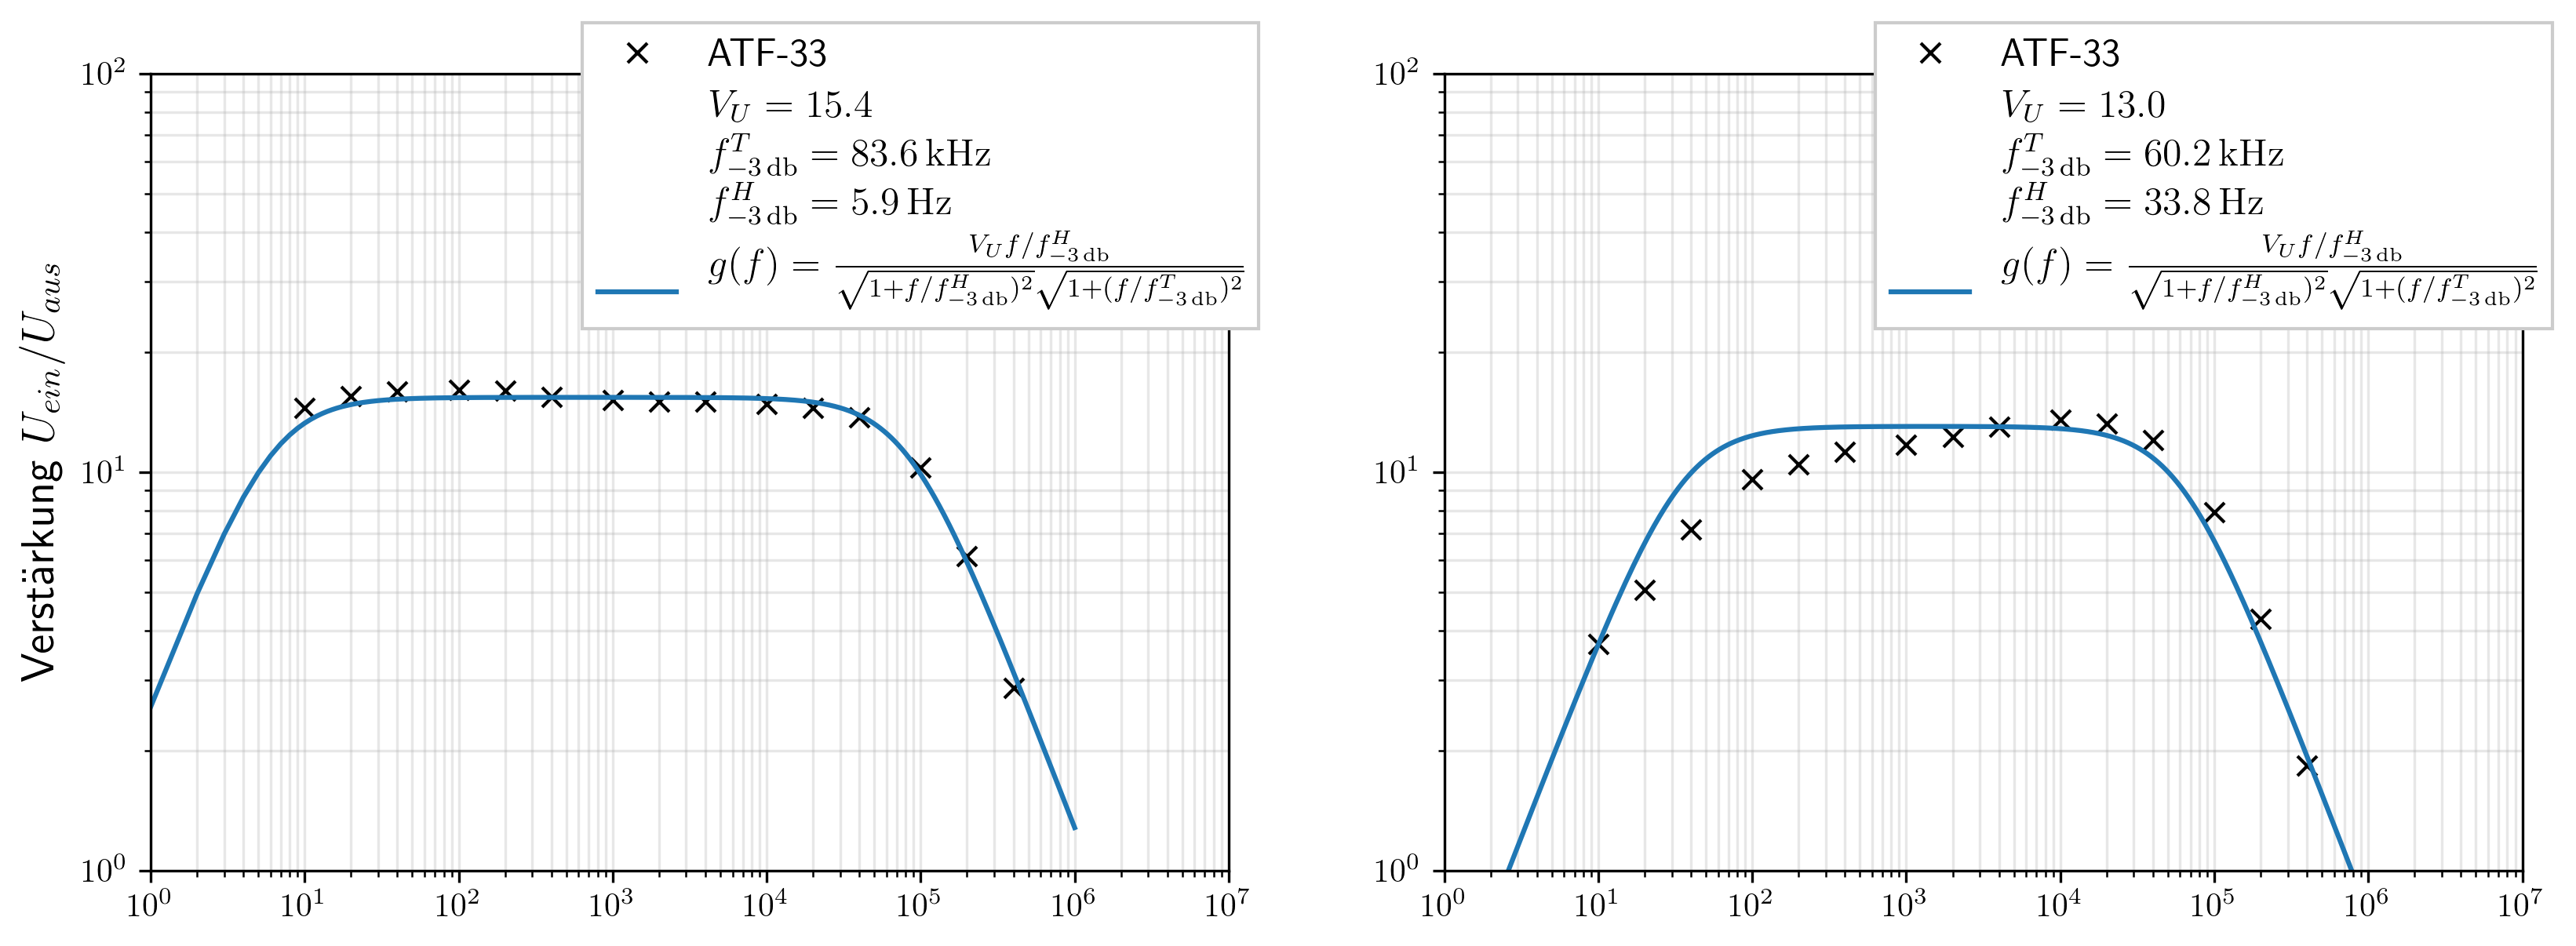
\includegraphics[width=\textwidth]{./fig/Gain/G33.png}
\captionof{subfigure}{Verstärkung der kalten Elektronik unter Verwendung des HEMTs ATF-33143\cite{ATF-33143}. Links: Verstärkung bei Raumtemperatur ($\SI{291}{\kelvin}$) und einer Biasspannung von $\SI{-0.6}{\volt}$. Rechts: Verstärkung bei flüssig Stickstoff Temperatur ($\SI{77}{\kelvin}$) und einer Biasspannung von $\SI{-1}{\volt}$.}
\label{subfig:33}
\end{minipage}
\vspace{0.5cm}
\begin{minipage}[c]{\textwidth}

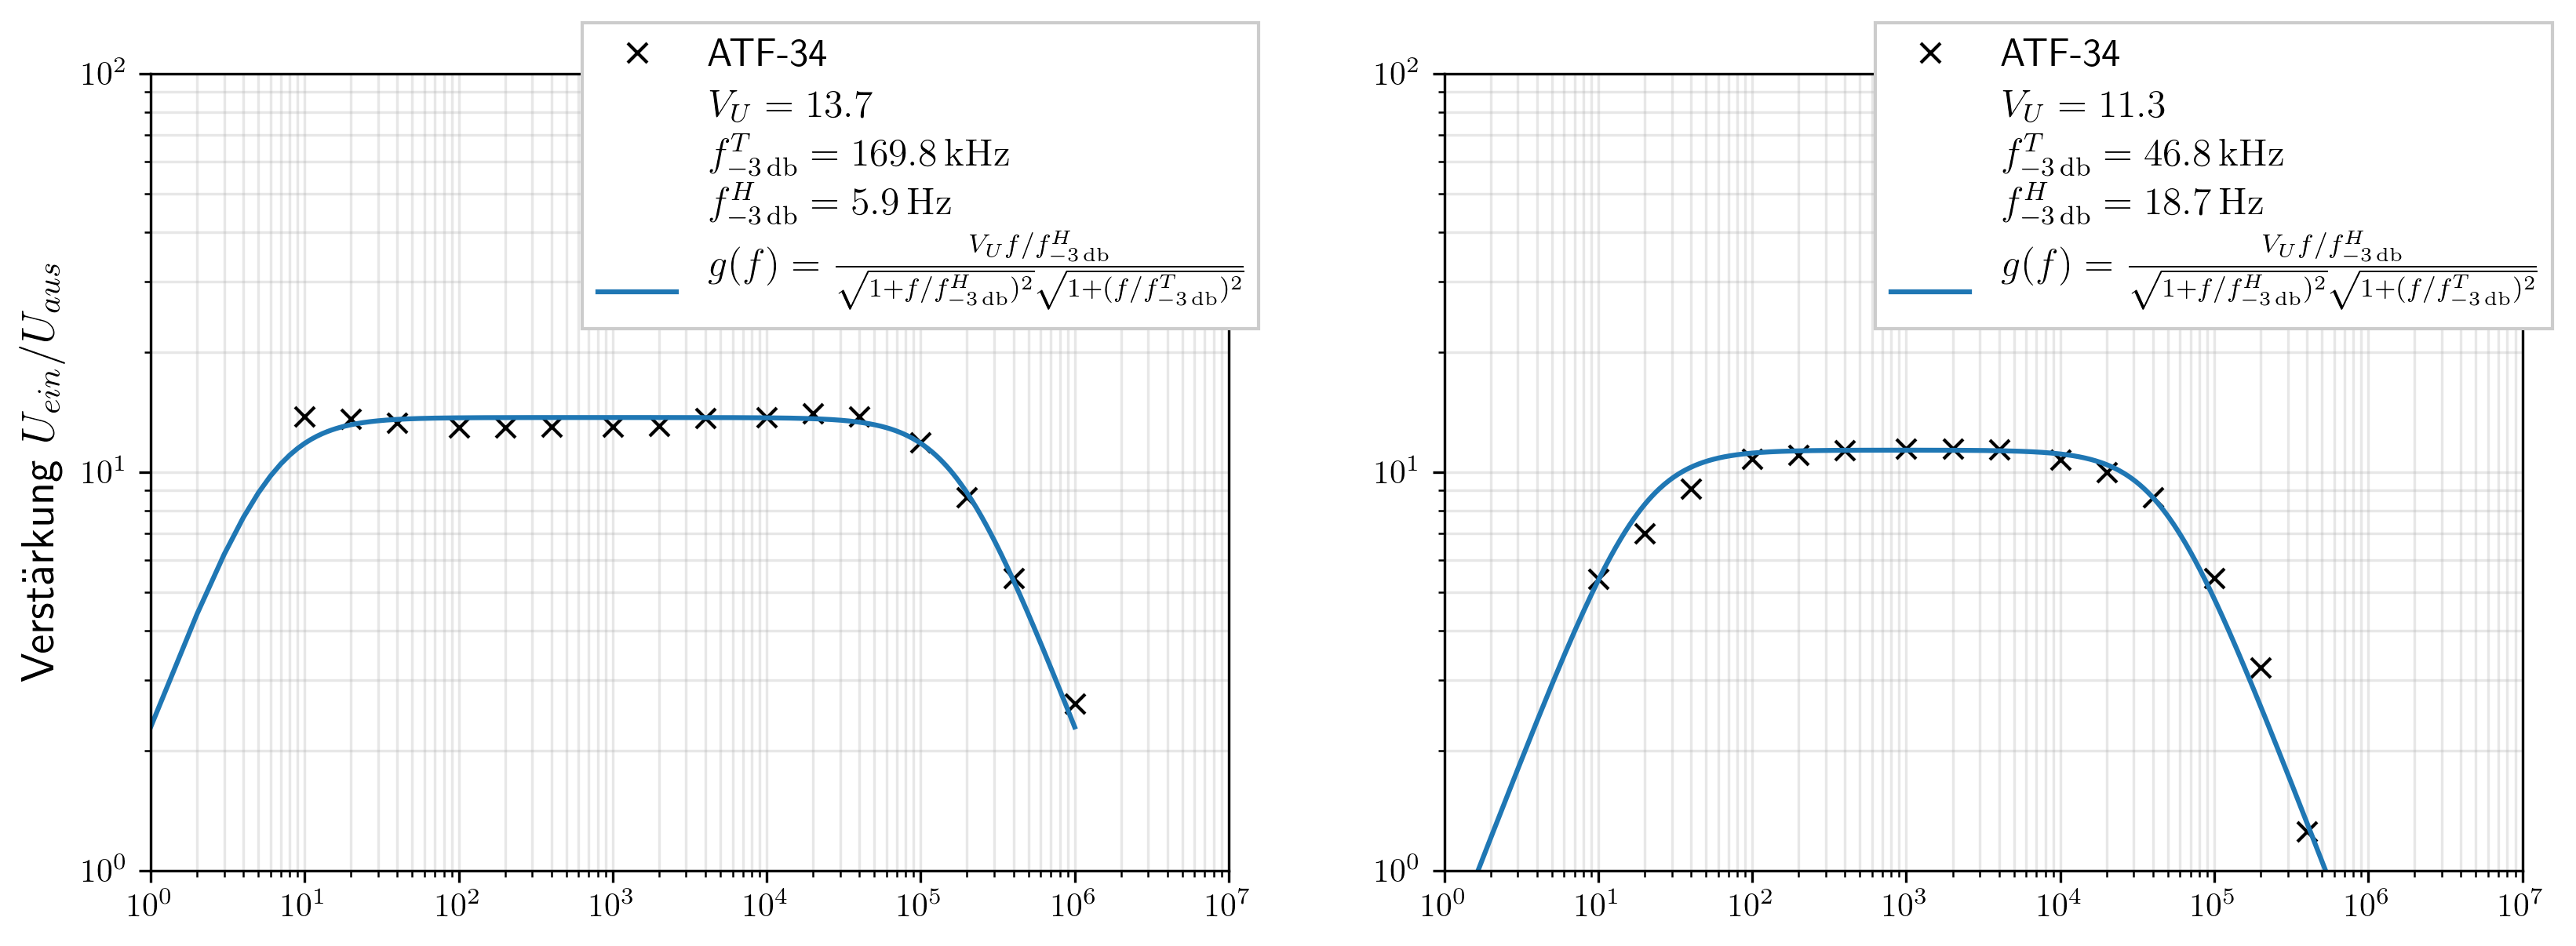
\includegraphics[width=\textwidth]{./fig/Gain/G34.png}
\captionof{subfigure}{Verstärkung der kalten Elektronik unter Verwendung des HEMTs ATF-54143\cite{ATF-34143}. Links: Verstärkung bei Raumtemperatur ($\SI{291}{\kelvin}$) und einer Biasspannung von $\SI{-0.74}{\volt}$. Rechts: Verstärkung bei flüssig Stickstoff Temperatur ($\SI{77}{\kelvin}$) und einer Biasspannung von $\SI{-0.94}{\volt}$.}
\label{subfig:34}
\end{minipage}
\vspace{0.5cm}
\begin{minipage}[c]{\textwidth}

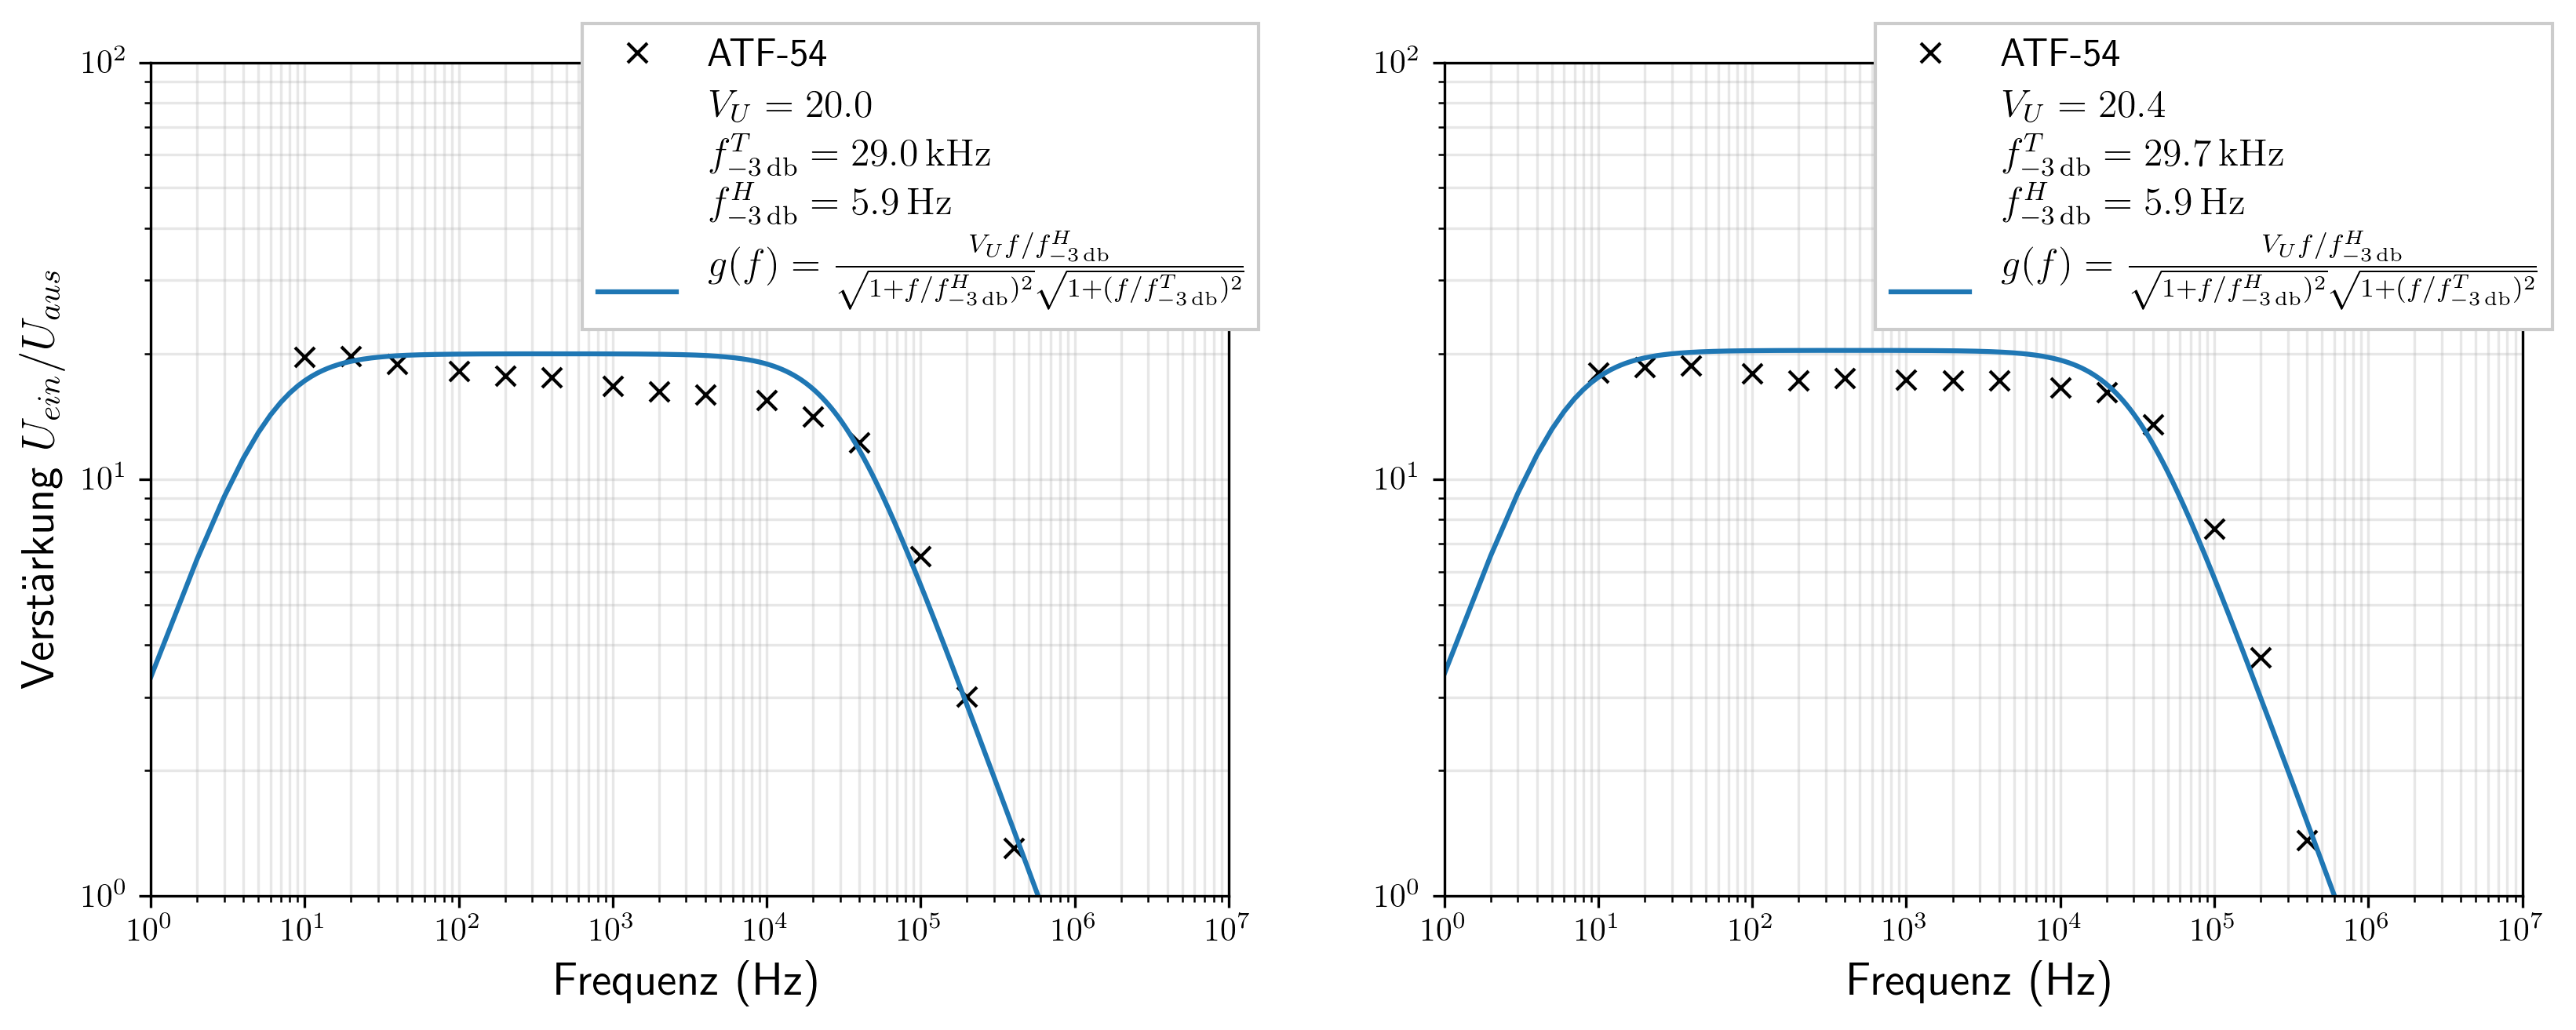
\includegraphics[width=\textwidth]{./fig/Gain/G54.png}
\captionof{subfigure}{Verstärkung der kalten Elektronik unter Verwendung des HEMTs ATF-54143\cite{ATF-54143}. Links: Verstärkung bei Raumtemperatur ($\SI{291}{\kelvin}$) und einer Biasspannung von $\SI{0.26}{\volt}$. Rechts: Verstärkung bei flüssig Stickstoff Temperatur ($\SI{77}{\kelvin}$) und einer Biasspannung von $\SI{0.38}{\volt}$.}

\captionof{figure}{An die Daten (schwarz) ist die Übertragungsfunktion angepasst (blau). Die Konstante $A$ gibt die Verstärkung im konstanten Bereich an. Das Inverse der Konstanten B die Grenzfrequenz des Tiefpass und das Inverse der Konstanten C die Grenzfrequenz des Hochpass.}
\label{fig:Gain}
\end{minipage}
\end{minipage}
\clearpage

Zu sehen ist, dass die aus den Daten ermittelte Grenzfrequenz des Tiefpass am Ausgang in allen Fällen ungefähr einen Faktor $10$ kleiner ist als die erwartete von $\SI{130}{\kilo\hertz}$ entsprechend Gl. \eqref{eq:AusgangTiefpass}.
Dies könnte auf die in der Theorie nicht berücksichtige Kapazität der Kabel zurückzuführen sein, welche parallel zur Kapazität $C_o$ erscheint.
Um diesem Effekt entgegen zu wirken kann der Widerstand $R_o$ kleiner gewählt werden.

Der Effekt des Hochpasses ist nicht zu sehen, da die aufgenommenen Daten nur bis zu einer minimalen Frequenz von $\SI{10}{\hertz}$ gehen.
Daher wurde die aus der Theorie vorhergesagte Grenzfrequenz verwendet.
Ausgenommen davon sind die beiden HEMTs ATF-34143 und ATF-33143, welche beide im Kalten eine deutlich höhere Grenzfrequenz des Tiefpass aufweisen.

\begin{figure}[!b]
\begin{center}
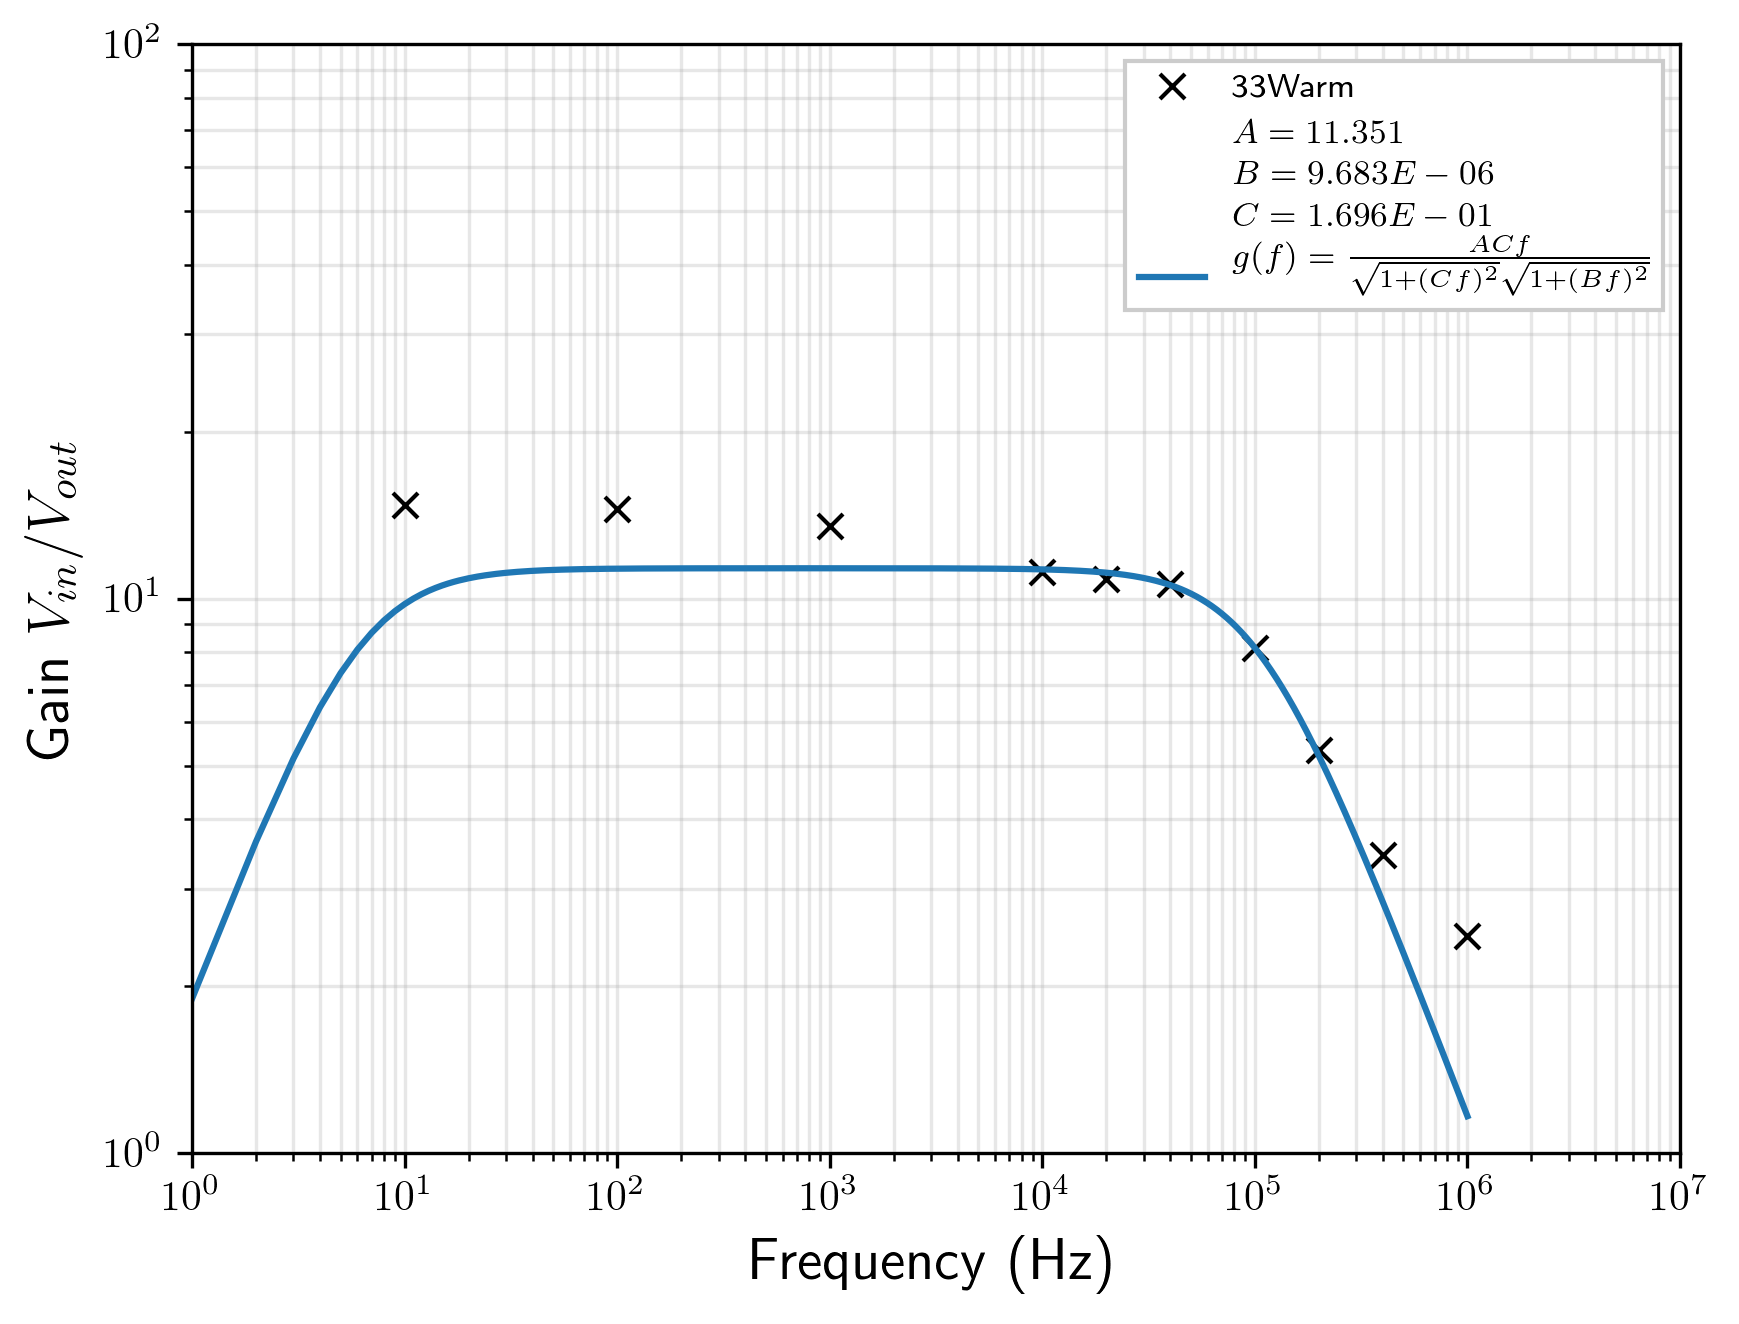
\includegraphics[width=0.65\textwidth]{./fig/Gain/G33WarmMarch21.png}
\vspace{-0.5cm}
\caption{Verstärkung des HEMTs ATF-33143 bei geschlossenen Relais, einem Drainwiderstand von $R_d = \SI{192}{\Omega}$ und einer Biasspanung von $\SI{-0.65}{\volt}$.}
\label{fig:33WarmGain100}
\end{center}
\end{figure}

Die Verstärkung aller drei HEMTs liegt in der Größenordnung von $10$ und ändert sich nur minimal mit der Temperatur.
Die aus der Theorie erwartete Verstärkung gegeben durch Gl. \eqref{eq:amp} liegt allerdings deutlich höher bei $200\-- 400$ je nach HEMT.
Dies könnte daran liegen, dass die HEMTs am Rand ihres Ausgangskennlinienfeldes betrieben werden, das heißt mit deutlich weniger Strom als sie konzipiert sind.
Um weiter in die Mitte des Kennlinienfeldes zu gelangen muss der Drainwiderstand $R_d$ herabgesetzt werden.
Die Abbildung \ref{fig:33WarmGain100} zeigt die Verstärkung bei einem Drainwiderstand von $R_d=\SI{192}{\Omega}$.
Zu sehen ist, dass die Verstärkung beinah unverändert in der Größenordnung von $10$ bleibt die aus der Theorie erwartete Verstärkung allerdings auf $20 \-- 40$ runter geht.
Außerdem geht die verbrauchte Leistung hoch auf $\SI{26}{\milli\watt}$.

Ein weiterer Grund kann der Frequenzbereich sein indem die HEMTs verwendet werden.
Eigentlich sind diese handelsüblichen HEMTs für den hochfrequenten Bereich von $\SI{500}{\mega\hertz}\--\SI{10}{\giga\hertz}$ konzipiert.
Daher haben sie auch sehr kleine Gate-Drain und Gate-Source Kapazitäten.

Die CNRS HEMTs dagegen sind speziell für den niederfrequenten Bereich und niedrigen Leistungsverbrauch ausgelegt.
Mit diesen konnte eine deutlich höhere Verstärkung erreicht werden \cite{Phipps:2016mwv}.
Da diese allerdings über deutlich größere Eingangskapazitäten verfügen, kann nicht länger der in Abschnitt \ref{sec:Amp} beschriebene Miller-Effekt vernachlässigt werden.
In diesem Fall kann statt einem Common-Source Verstärker zum Beispiel eine Kaskodenschaltung verwendet werden \cite{Gray}.

In Abbildung \ref{fig:54RClosed} ist die Verstärkung des HEMTS ATF-54143 bei offenem Relais gezeigt.
Dieser ist der einzige HEMT dessen Leckstrom bei flüssig Stickstoff Temperaturen klein genug ist, sodass die Biasspannung über einen längeren Zeitraum gehalten wird.
Der Effekt des Hochpass entfällt und die Übertragungsfunktion wird zu
\begin{equation}
U_a = U_e \frac{V_U}{\sqrt{1+(f/f^T_{-3\,\mathrm{db}})^2}}.
\end{equation}

\begin{figure}[!t]
\begin{center}
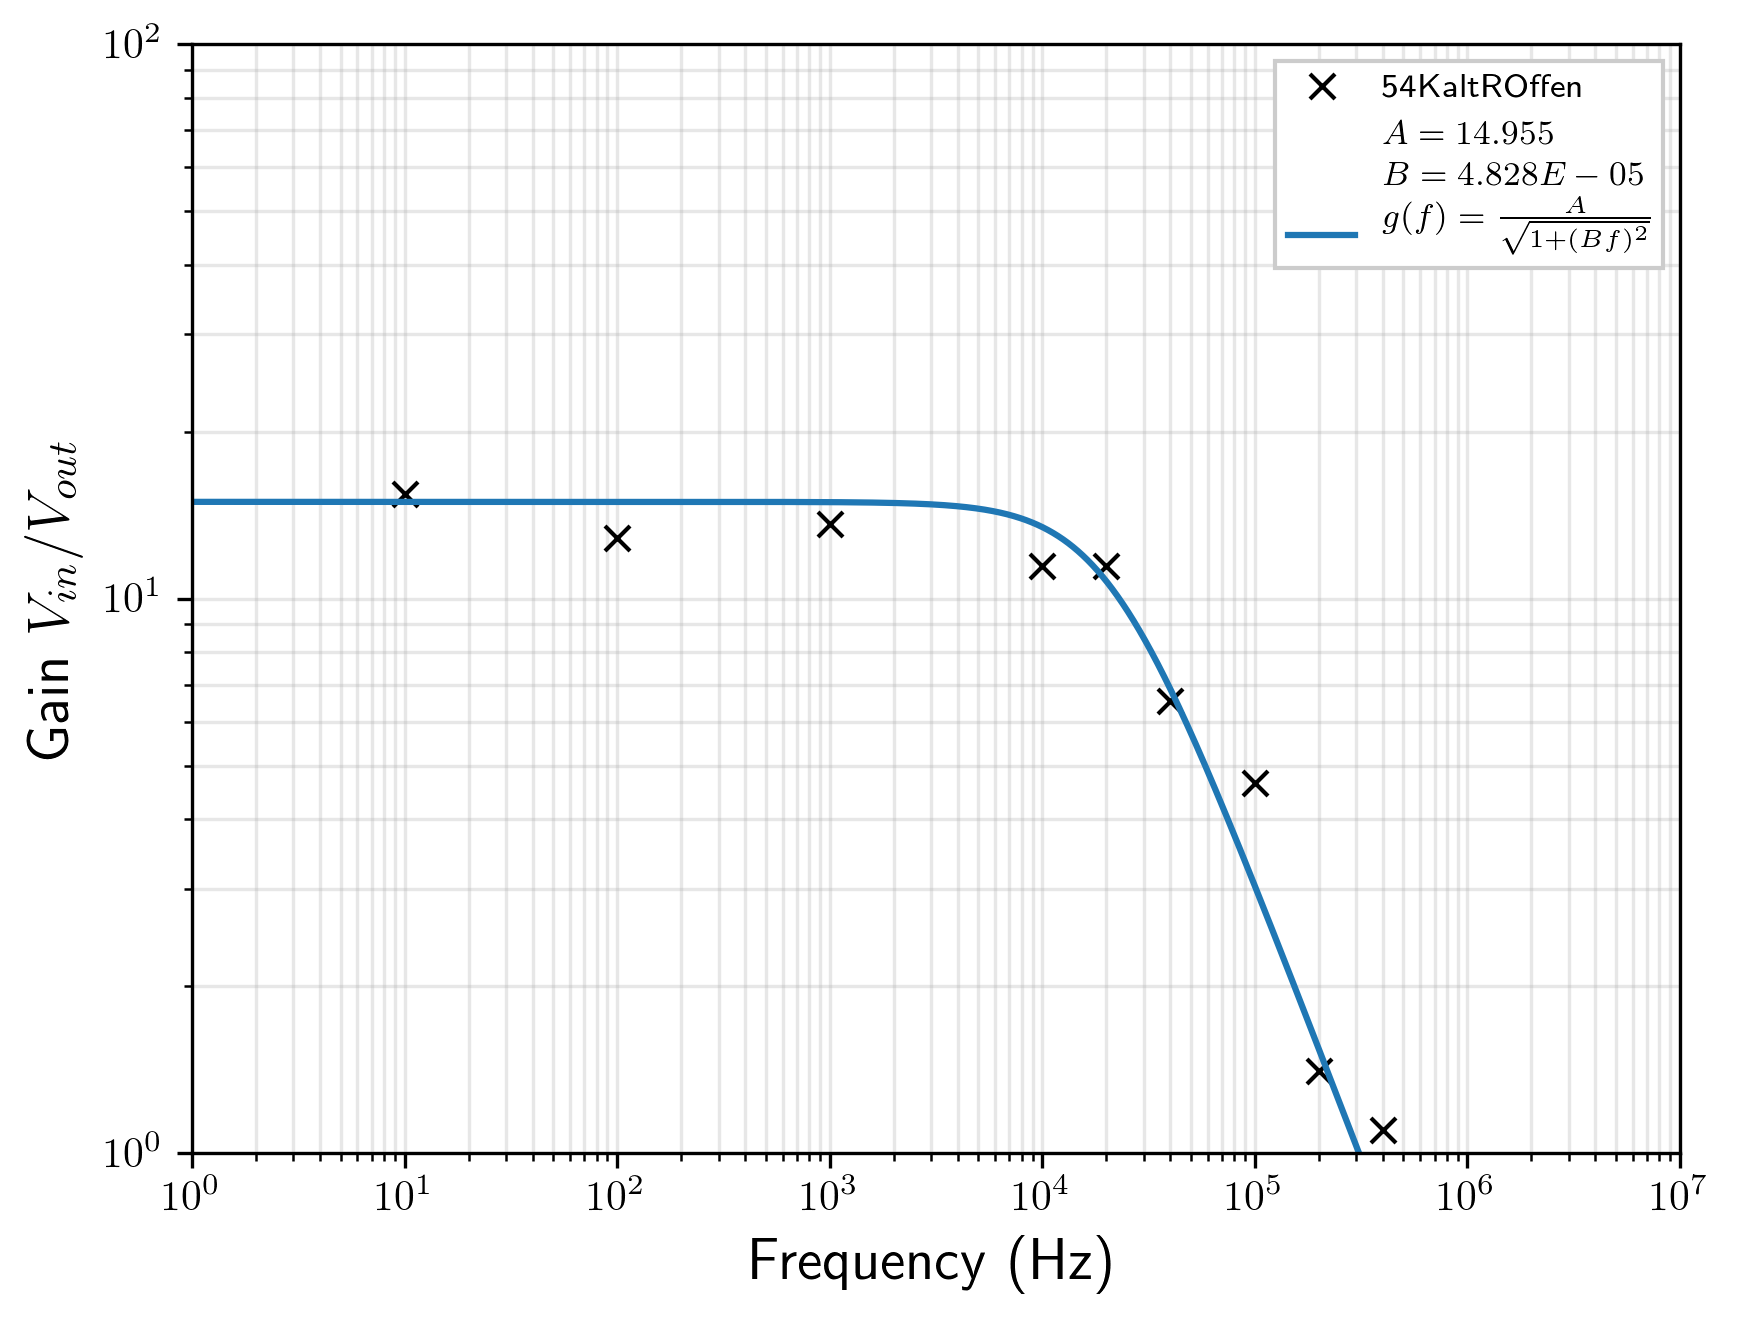
\includegraphics[width=0.65\textwidth]{./fig/Gain/G54ColdROpen.png}
\vspace{-0.5cm}
\caption{Verstärkung des HEMTs  ATF-54143 bei offenem Relais und einer Biasspannung von $\SI{0.371}{\volt}$.}
\label{fig:54RClosed}
\end{center}
\end{figure}

Bei bekannter Verstärkung lässt sich Eingangskapazität des Verstärkers $C_{amp}$ bestimmen und damit die gesamte Eingangskapazität der Schaltung $C_{ges}$.
Gemäß Gl. \eqref{eq:EingangsC} und \eqref{eq:Camp} gilt
\begin{equation}
C_{ges}=C_d+ C_{int} + C_{amp} + C_{Kabel} = \SI{30}{\pico\farad} + \SI{4,7}{\pico\farad} + \SI{5.8}{\pico\farad} + \SI{63,75}{\pico\farad} = \SI{104,25}{\pico\farad}.
\end{equation}
Die Kapazität der Kabel stammt von dem $\SI{1,5}{\meter}$ langen Koaxialkabel welches zum Anschluss an den Signalgenerator verwendet wurde.
Die restlichen Kabel werden entweder durch große Widerstände bzw. Relais getrennt und die Leiterbahnen auf der kalten Elektronik sind vernachlässigbar kurz.


